\documentclass[10pt]{article}
\usepackage[margin=1in]{geometry} 
\usepackage{amsmath,amsthm,amssymb, graphicx, multicol, array}\usepackage[utf8]{inputenc}
\usepackage{fancybox}
\usepackage{setspace}
\usepackage{adjustbox}
\usepackage{minted}
\usepackage{biblatex}
\newcommand{\half}{\frac{1}{2}}
\newcommand{\xyz}{\begin{pmatrix}x\\y\\z\end{pmatrix}}
\newcommand{\f}[1]{\mathbf{#1}}
\newcommand{\A}{\mathcal{A}}
\newcommand{\B}{\mathcal{B}}
\newcommand{\R}{\mathbb{R}}
\newcommand{\Z}{\mathbb{Z}}
\newcommand{\C}{\mathbb{C}}
\newcommand{\N}{\mathbb{N}}
\newcommand{\Rsp}{\mathbb{R}^*_+}
\newcommand{\dub}[1]{\mathbb{#1}}
\newcommand{\D}{\partial}
\newcommand{\Img}{\mathrm{Im}}
\newcommand{\bigO}{\mathcal{O}}
\newcommand{\inv}{^{-1}}
\newcommand{\supno}[1]{||#1||_\infty}

\newcommand{\gaute}[1]{{\color{red} #1}}

\bibliography{references}


\title{Tensor Factorizations Course Project}
\author{Gaute Johannessen}
\date{June 2025}
\newenvironment{problem}[2][Problem]{\begin{trivlist}
\item[\hskip \labelsep {\bfseries #1}\hskip \labelsep {\bfseries #2.}]}{\end{trivlist}}
\newenvironment{exercise}[2][Exercise]{\begin{trivlist}
\item[\hskip \labelsep {\bfseries #1}\hskip \labelsep {\bfseries #2.}]}{\end{trivlist}}


\begin{document}
\maketitle

\section*{Part 1}
In this part we analyze a third-order tensor using a CP-model.
Our dataset $\ten{X}\in \R^{28 \times 251 \times 21}$
\gaute{Finish intro}


\subsection*{Background and Method}

We fit the CP model to the data using the \texttt{cp\_wopt} function from the Tensor Toolbox \cite{tentool}.
The reason we have selected this function, is due to the data having missing values.
Indeed, the function allows us to pass a weight tensor $\ten{W}$ as an argument, where we define $\ten{W}$ as in (\ref{eq:weight_matrix}).


\begin{equation}
\mathcal{W}_{i,j,k} = \begin{cases}
    1 \ \text{if} \ \ten{X}_{i,j,k} \ \text{is in the dataset,} \\
    0 \ \text{if} \ \ten{X}_{i,j,k} \ \text{is missing.}
\end{cases}
\label{eq:weight_matrix}
\end{equation}

\begin{equation}
    \min_{ \mathcal{\hat{X}}} \frac{1}{2} ||\mathcal{W} * (\mathcal{X} - \mathcal{\hat{X}})||^2 \text{  where } \mathcal{\hat{X}} = \sum_{r = 1}^{R} \lambda_r \mathbf{a}_r \circ \mathbf{b}_r \circ \mathbf{c}_r
    \label{eq:cp}
\end{equation}

We use this weight matrix to define the expression we want to optimize, described in (\ref{eq:cp}).
This is the same description of the CP model as used in \textcite{tensor-review}, with the added weight tensor for handling the missing data, described in \textcite{cp-wopt}.
In (\ref{eq:cp}), the norm used is the Frobenius norm for tensors, $*$ denotes the element-wise Hadamard product, and $\circ$ denotes an outer vector product.
This weight matrix formulation allows us to fit the model based on all our data, without having to replace the missing data with any synthetic replacements.

Having set up the CP-model (\ref{eq:cp}), we now need a way to fit the optimal $\ten{\hat{X}}$, i.e. finding the rank $R$, weights $\boldsymbol{\lambda}$, and matrices $A, B$ and $C$.
Note that $\f{a}_r$ is the $r$'th column of $A$, and similar for $\f{b}_r$ in $B$ and $\f{c}_r$ in $C$.
The \texttt{cp\_wopt} algorithm precomputes $\ten{Y} = \ten{W} * \ten{X}$ for efficiency, and computes the gradients of the function with respect to the matrices $A, B$ and $C$ respectively.
The gradient of $f$ with respect to $A$ is included in (\ref{eq:gradA}) as an example \cite{cp-wopt}.
Here, $f$ refers to the function to be minimized as described in \ref{eq:cp}, $\mathcal{Z}$ is defined as $\ten{Z} = \ten{W} * \ten{\hat{X}}$, $\odot$ denotes the Khatri-Rao matrix product (see \textcite{tensor-review}, p. 462), and $Z_{(n)}$ denotes the $n$-mode matricization of the tensor $\ten{Z}$.
\begin{equation}
    \frac{\partial f}{\partial A} = (Z_{(1)} - Y_{(1)})(C \odot B) 
    \label{eq:gradA}
\end{equation}
For the optimization step, we use the L-BFGS-B algorithm, which is a version of the Limited-memory Broyden–Fletcher–Goldfarb–Shanno algorithm (L-BFGS) made for solving large nonlinear optimization with simple bounds on the variables \cite{lbfgsb}.
This is the recommended optimization algorithm for the \texttt{cp\_wopt} function according to the Tensor Tooblox documentation.
We also impose a non-negativity constraint in all modes, as we expect the patterns in the underlying data to be non-negative.

As the loss-landscape of the model is expected to be non-convex, the initial values of the model used in fitting could affect the final result, e.g. if we start close to a local minima, we could converge to that instead of the global minima.
To ensure that we get a good/optimal model for the problem, we initialize the model multiple times, using random initialization, before we fit each of them.
For further analysis we will always keep the best model, that is the model with the lowest loss after its final iteration.



\gaute{Explain using multiple inits}

\gaute{Explain finding rank}

\gaute{Explain uniqueness}


\subsection*{Results}

\begin{figure}[H]
    \centering
    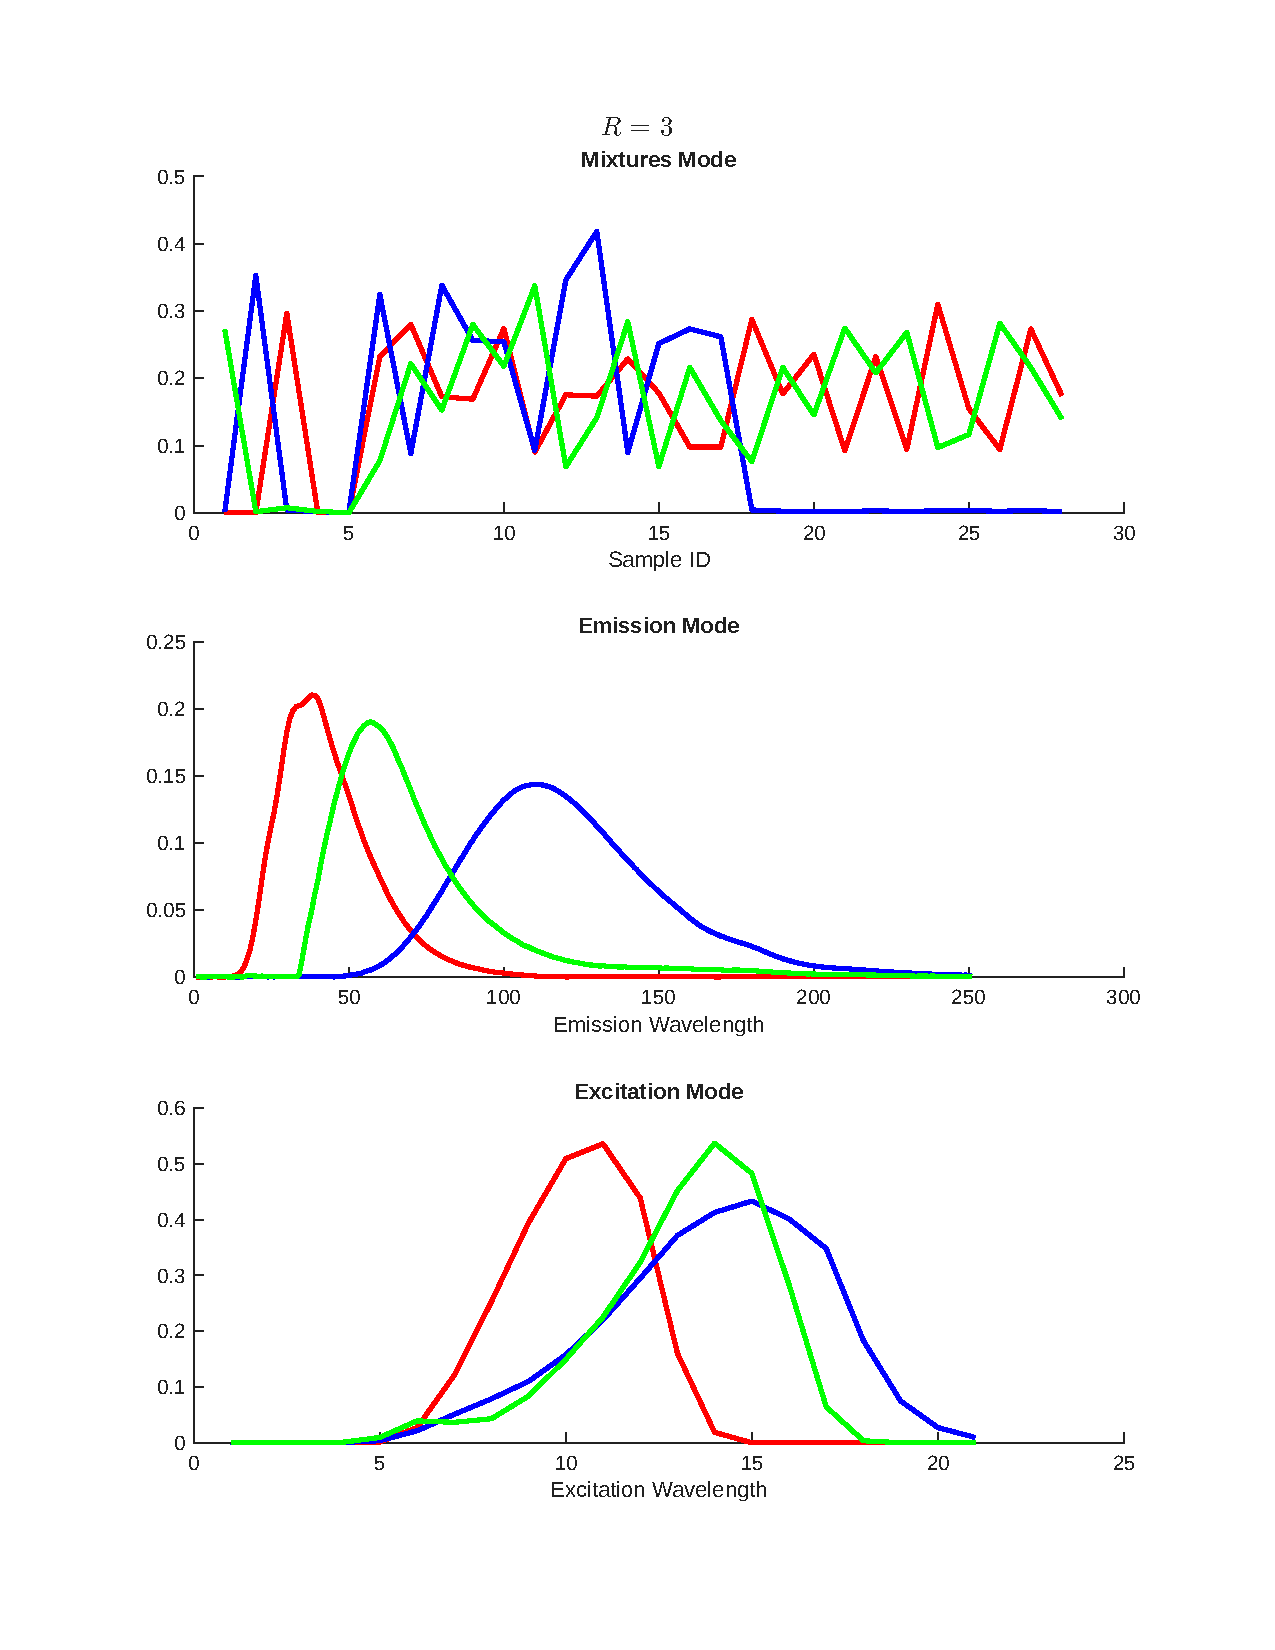
\includegraphics[trim = 2cm 5cm 2cm 5cm, clip, width=0.46\linewidth]{figures/factors_rank3.pdf}
    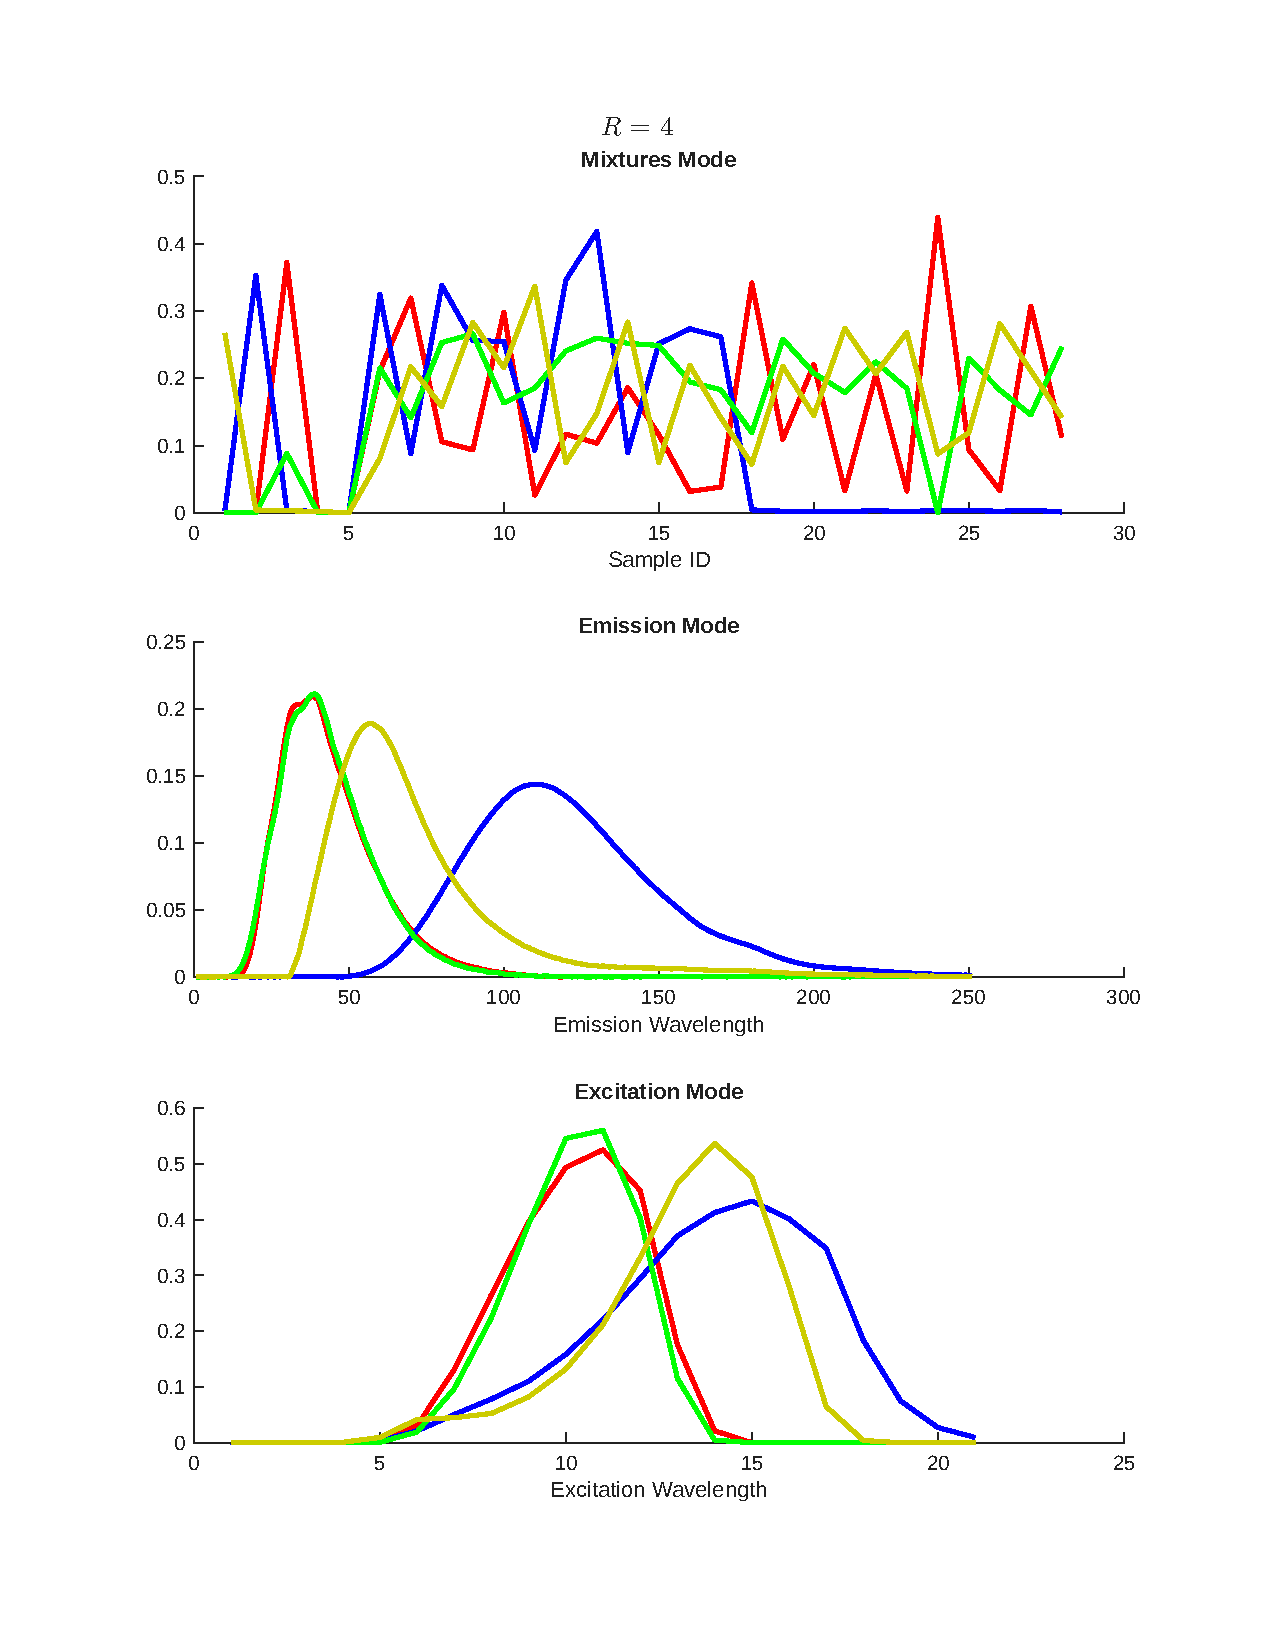
\includegraphics[trim = 2cm 5cm 2cm 5cm, clip, width=0.46\linewidth]{figures/factors_rank4.pdf}
    \caption{}
    \label{fig:plot_factors}
\end{figure}



\section*{Part 2}


We pre
\cite{framework}
\subsection*{Results and Discussion}

\gaute{Uniqueness results (in matlab terminal)}

\gaute{discuss results}

\begin{figure}[H]
    \centering
    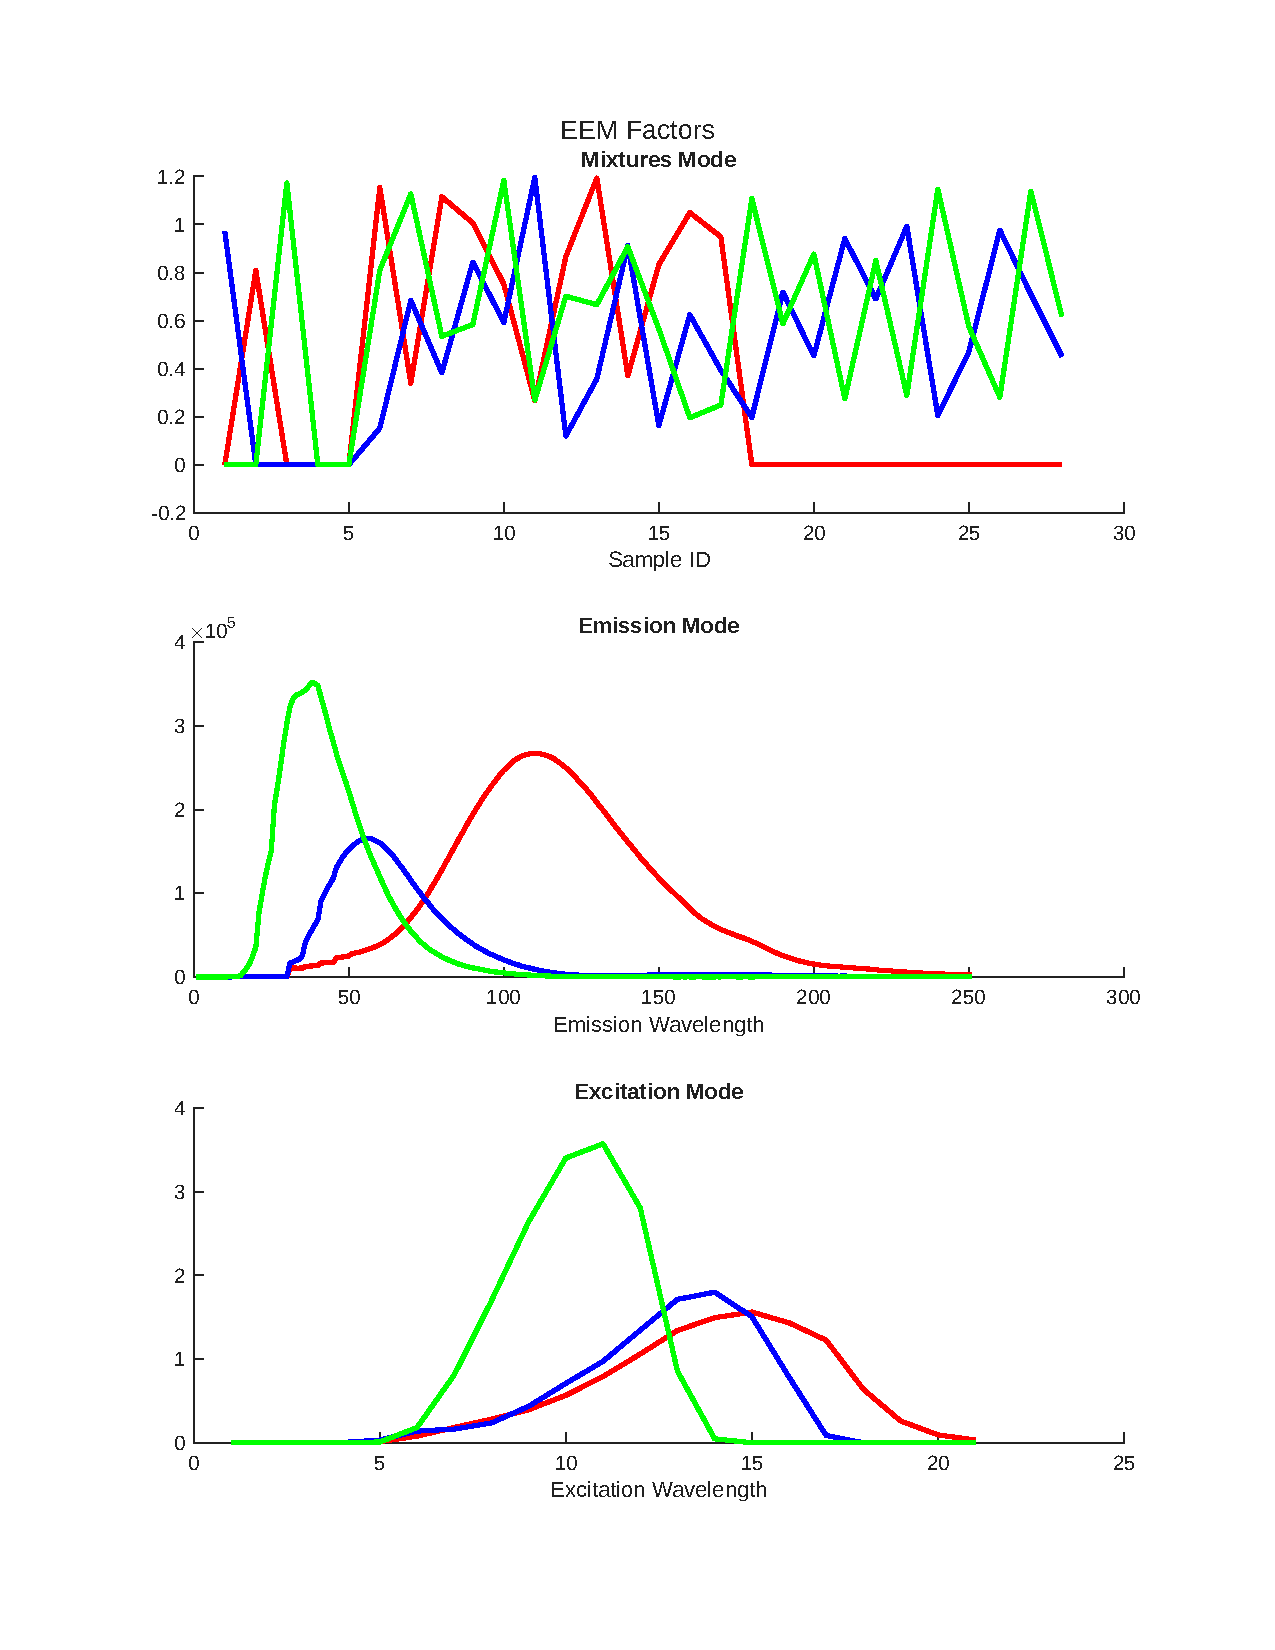
\includegraphics[trim = 2cm 2.5cm 2cm 1.9cm, clip, width=0.46\linewidth]{figures/factors_EEM Factors.pdf}
    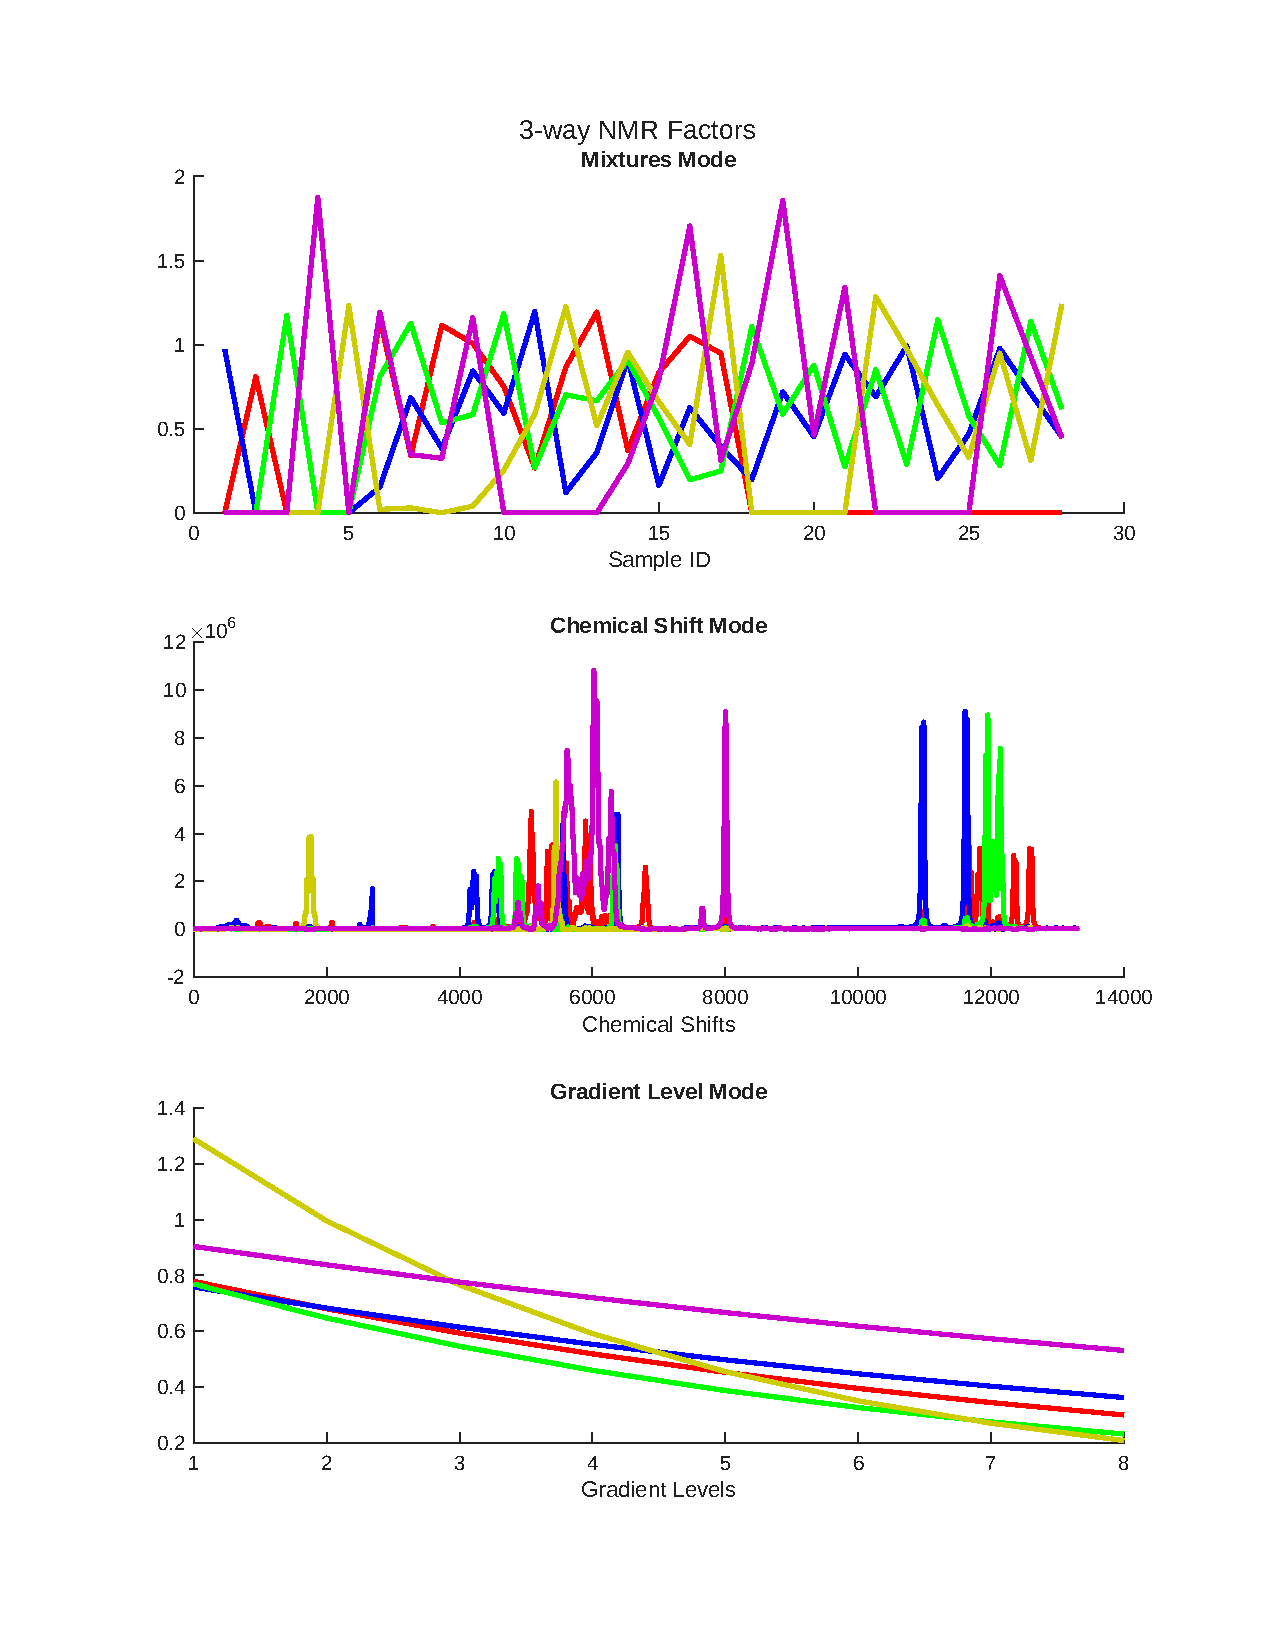
\includegraphics[trim = 2cm 2.5cm 2cm 1.9cm, clip, width=0.46\linewidth]{figures/factors_3-way NMR Factors.pdf}
    \caption{}
    \label{fig:plot_factors}
\end{figure}
\begin{figure}[H]
    \centering
    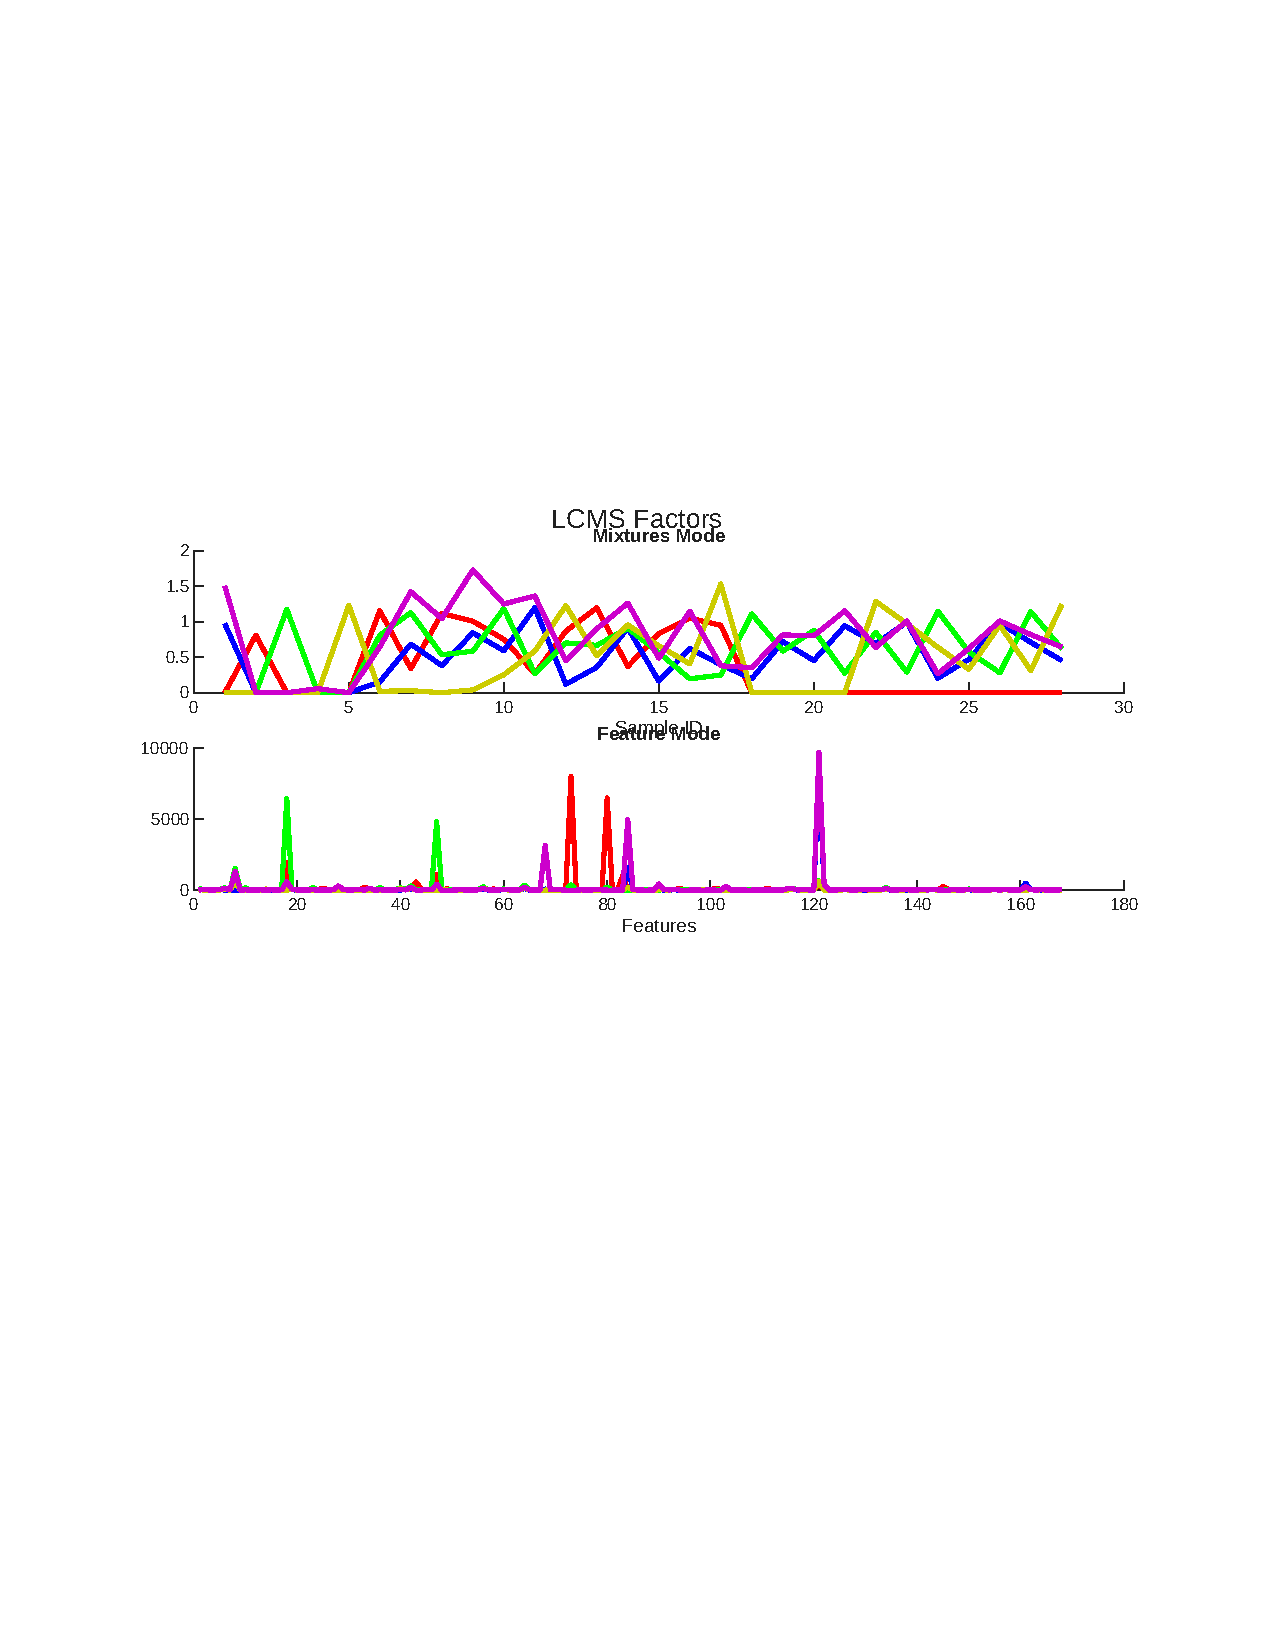
\includegraphics[trim = 2cm 10cm 2cm 1.9cm, clip, width=0.46\linewidth]{figures/factors_LCMS Factors.pdf}
    \caption{}
    \label{fig:plot_factors}
\end{figure}

\printbibliography
\end{document}

